\documentclass[11pt,a4paper]{article}
\usepackage{float}
\usepackage{verbatim}
\usepackage{subfig}
\usepackage[T1]{fontenc}
\usepackage[utf8]{inputenc}
\usepackage{geometry}
\usepackage{enumitem}
%\geometry{verbose,lmargin=2cm,rmargin=2cm, bmargin=2cm, tmargin=2cm}
\usepackage{wrapfig}
\usepackage{tikz}
\usetikzlibrary{decorations.markings}
\usepackage{calc}
\usepackage{wrapfig}
\usepackage{graphicx}
\usepackage{amssymb}
\usepackage{amsmath}
\usepackage{esint}
\usepackage{hyperref}
\usepackage{listings}
\hypersetup{
    colorlinks=true,
    linkcolor=blue,
    filecolor=magenta,
    urlcolor=cyan,
}
\usepackage{listings}
\lstset{ %
  backgroundcolor=\color{white},   % choose the background color; you must add \usepackage{color} or \usepackage{xcolor}; should come as last argument
  basicstyle=\footnotesize,        % the size of the fonts that are used for the code
  breakatwhitespace=false,         % sets if automatic breaks should only happen at whitespace
  breaklines=true,                 % sets automatic line breaking
  captionpos=t,                    % sets the caption-position to bottom
  commentstyle=\color{teal},    % comment style
  deletekeywords={...},            % if you want to delete keywords from the given language
  escapeinside={\%*}{*)},          % if you want to add LaTeX within your code
  extendedchars=true,              % lets you use non-ASCII characters; for 8-bits encodings only, does not work with UTF-8
  frame=single,                    % adds a frame around the code
  keepspaces=true,                 % keeps spaces in text, useful for keeping indentation of code (possibly needs columns=flexible)
  keywordstyle=\color{blue},       % keyword style
 % language=Python,                 % the language of the code
  morekeywords={*,...},           % if you want to add more keywords to the set
  numbers=left,                    % where to put the line-numbers; possible values are (none, left, right)
  numbersep=5pt,                   % how far the line-numbers are from the code
  numberstyle=\tiny\color{black}, % the style that is used for the line-numbers
  rulecolor=\color{black},         % if not set, the frame-color may be changed on line-breaks within not-black text (e.g. comments (green here))
  showspaces=false,                % show spaces everywhere adding particular underscores; it overrides 'showstringspaces'
  showstringspaces=false,          % underline spaces within strings only
  showtabs=false,                  % show tabs within strings adding particular underscores
  stepnumber=1,                    % the step between two line-numbers. If it's 1, each line will be numbered
  tabsize=2,                       % sets default tabsize to 2 spaces
  title=\lstname                   % show the filename of files included with \lstinputlisting; also try caption instead of title
}
\begin{document}



%\preprint{APS/123-QED}

\title{FYS2150 \\ Lab Report: Elasticity}% Force line breaks with \\

\author{Nicholas Karlsen}
% \email{nichoka@student.matnat.uio.no}

\date{\today}% It is always \today, today,
             %  but any date may be explicitly specified

\maketitle

\begin{abstract}
Determining the Young's modulus of a brass rod by measuring the deflection in three-point bending and determining its root frequency. Comparing the two methods and investigating if their results overlap.
\end{abstract}

%\tableofcontents

\section{\label{sect:intro}Introduction}
  This report contains the procedure, results and analysis of experiments performed in an attempt to determine the Young's modulus of a Brass rod. We performed two different methods for determining it experimentally; By suspending a varied load unto the rod whilst held up by two knives and determining the Young's modulus by the resulting deflection of the rod, and by listening for the root frequency emitted from the rod when struck by a hammer, both by ear and numerically by recording the audio and looking at the frequency domain of the data by Fourier transforming it.

  The goal was to obtain two independent values for the Young's modulus whose values overlap within the uncertainties of the experiments, suggesting an accurate result of Young's modulus. 

\section{\label{sect:theory}Theory}
  \subsection{Three-point bending}
  From the Euler-Bernoulli beam theory \cite{3pt}, it follows that the deflection of a beam supported by two points of distance $l$ and a load $mg$ halfway between the two knives is given by
  \begin{equation}
    h(m) = \frac{mgl^3}{48EI}
    \label{eqn:hm_exp}
  \end{equation}
  Where $E$ denotes the Young's modulus \cite{ymodul} of the beam and $I$ the second moment area given by 
  \begin{equation}
    I = \frac{\pi d^4}{4\cdot 2^4}
  \end{equation}
  Where $d$ denotes the diameter of the beam.
  \newline
  Further, Eqn. \ref{eqn:hm_exp} can be rewritten in the following way
  \begin{equation}
    E = \frac{4l^3g}{3\pi |A|d^4}
    \label{eqn:E_deflection}
  \end{equation}
  Where $A \equiv h(m)/m$, which can be obtained as the gradient from a linear fit on the data gathered when varying the load subjected and on the beam and recording the resulting deflection. Which gives the following relationship
  \begin{equation}
    h(m) = Am + B
  \end{equation}
  
  \subsection{Sound emitted from a brass rod}

  When struck on its axial side, a metallic rod of certain specifications emit an audible sound made up of signals of varying frequencies. The most audible of which is the root tone. The root tones' frequency is determined by Eqn. \ref{eqn:root_tone} where $d$ denotes the diameter of the rod, $M$ its mass, $L$ its length and $E$ its Young's modulus.

  \begin{equation}
    f = \frac{d}{4}\sqrt{\frac{\pi E}{M L}}
    \label{eqn:root_tone}
  \end{equation}

  \subsection{Beats}
    \begin{equation}
      f_S = \frac{|\omega - \omega'|}{2}\frac{1}{2\pi}
      \label{eqn:beats}
    \end{equation}
    When two signals of similar frequencies, $\omega, \omega'$, superimpose, there is an audible beat of a certain frequency, $f_S$. The frequency of this audible beat is given by Eqn. \ref{eqn:beats}, and becomes lower the smaller the difference in frequencies between the two signals.

  \subsection{Errors}
    When performing arithmetic operations on recorded data, the uncertainty in the data must also carry over to the derived results. How these uncertainties are propagated in different operations can be found in Practical Physics \cite{squires}.


\section{\label{section:experimental}Experimental Procedure}
  \subsection{Three-point flexural test}

    \begin{figure}[H]
      \centering
      \subfloat[][]{
        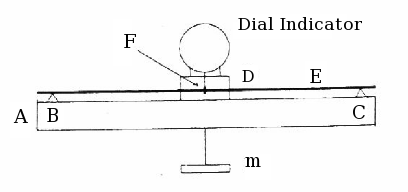
\includegraphics[width=9cm]{scripts/figs/aparatus1.png}
          \label{fig:aparatus1}}
      \subfloat[][]{
        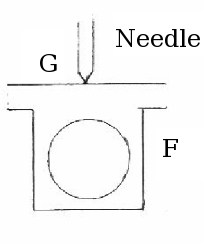
\includegraphics[width=4cm]{scripts/figs/aparatus1cs.png}
          \label{fig:aparatus1cs}}
      \center
      \caption{(a) shows the apparatus used for measuring the deflection of a rod and (b) a cross section of the  apparatus at point F.}
      \label{fig:exp_1}
     \end{figure}

    Using Fig. \ref{fig:aparatus1} as a reference; First, we ensured that the needle of the Baker\footnote{I did not take note of the model number of the particular dial gauge that was used during the lab. While working on this report, i have become aware that each Baker dial gauge is individually calibrated. Therefore, i have no values for the instrumental error in the deflection measurements.} dial gague was centered between B and C. We did this by measuring the distance from F to B and F to C, making adjustments such that the difference was sufficiently small. The distances were measured using a measuring tape of type Lufkin pee wee 2m Y612CM with an uncertainty of $\pm 0.1$cm. The brass rod, A, was laid on the "knives" B and C, such that the overhang of the rod from B and C were equal. In the middle of the rod, there was a ring attached, as shown in Fig. \ref{fig:aparatus1cs}. The flat surface of the ring was in contact with the needle of the dial gauge at G. In order to ensure that the flat surface of the ring was at right angle with the needle, we turned the rod such that the reading of the dial gauge would be at a minimum, as the skewer the surface, the greater the reading. This process was repeated at the start of every attempt of the experiment.

    After having prepared the apparatus, three masses of roughly $0.5$g, $1$kg and $2$kg which we denoted $m_a, m_b$ and $m_c$ respectively. They were placed carefully in the tray denoted m in Fig. \ref{fig:aparatus1}, in different combinations so that we would get readings for the deflection of the rod at $\approx \{0.5, 1, 1.5, 2, 2.5, 3, 3.5\}$kg, recorded by reading the dial gauge.

    Due to seemingly disturbing the system significantly when adding masses, we were worried that there might be a significant systematic error in the experiment. So we opted to repeat the readings in this experiment several times in order to investigate if the data in the later readings (when the system had been disturbed multiple times in succession) had an increase in its deviation.

    Lastly, the distance between the knives, $l_{B, C}$, was measured using the measuring tape and a micrometer of type Moore \& Wright 1965 MI with uncertainty $\pm0.01$mm. The measuring tape was used to measure the distance between the outer edges of the "knives" at B and C, $l_{B\, outer}$, $l_{C\, outer}$. The micrometer was then used to measure the knives thickness $l_{knife}$, which was needed as the contact points between the rod and the knives are (assumed) at the middle of the identical knives. Since there are two contact points, $l_{B\,outer, C\, outer}$ - $l_{knife}$ = $l_{B, C}$
    
  \subsection{Measuring the speed of sound in the rod}
      The brass rod, with a ring attached to it (same as before), was laid to rest on the flat side of the ring on a solid surface such that the rod is held up by the ring, and nothing else. We also made sure that the rod was not to be disturbed in any way while it was vibrating. When hit with a hammer, it will emit a sound consisting of different frequencies. Following are the two different methods we used for determining the root frequency of the rod.
      During both experiments, we ensured there were no significant noise pollution during our recording (By which i mean people performing the same experiment as us).
      \subsubsection{By hearing for beats}
        A speaker was connected to a signal generator. We started the signal generator at 1200Hz and hit the brass rod with a plastic hammer on the the flat surface on one end of the rod. By ear, there was an audible beat due to the superposition of the two signals. We adjusted the signal generator such that the the frequency of the beat was minimized, and there was essentially no audible difference between the two signals. We did this by trying above and below where we thought the root frequency was, eventually zeroing in on a value.

      \subsubsection{By Fourier transform}
        A USB microphone was placed close to the rod, and faced towards it. The microphone was connected to a computer running matlab, with a script that collects audio data from it and Fourier transforms it using a fast Fourier transform, FFT. The recordings made were made with a sampling frequency of $8\times1024$ Hz and varying durations. As before, we hit the rod using a plastic hammer and recorded the data. A total of 7 recordings were made.

      \subsection{Other measurements}
        \subsubsection{Mass}
          In order to accurately measure the mass of the rough loads and the rod, the balance scale (Ohaus triple beam balance) which we used had to be calibrated. We did this by weighing a set of three reference weights on the scale, and comparing their measured value to the measured value of the rough loads and the rod using a linear fit.When placing the masses on the scale, we made sure to position the masses in the center of the scale plate and not take a reading until the needle of the balance scale was not sufficiently stable.

        \subsubsection{Length and thickness of the rod}
          The length of the rod was measured using the measuring tape, and the thickness using the micrometer. In order to accurately determine the thickness, accounting for any irregularities in the rod due to deformation etc. The thickness was measured several times in different places on the rod, so that we could calculate the mean thickness.



\section{\label{sect:results}Results}
  
  \subsection{Length and mass measurements}
    
    \begin{table}[H]
      \center
      \caption{Mass of rough load and reference}
      \begin{tabular}{ | l | l | l | l | l |}
        \hline
        Stated mass   & Measured reference load   & Measured rough load & Measured ring & Measured rod + ring \\ \hline
        $500$g        & $500.0$g             & $500.1$g &   &  \\ \hline
        $1000$g       & $999.9$g             & $1000.3$g &  &  \\ \hline
        $2000$g       & $2000.1$g            & $2000.5$g &  &  \\ \hline
        n/a           &  &  & 34.4g & 2482.5g
        \\ \hline
      \end{tabular}
      \label{tab:masses}
    \end{table}

    \begin{table}[H]
      \center
      \caption{Calibrated masses}
      \begin{tabular}{ | l | l | l |}
        \hline
        Stated mass & Calibrated rough load & Calibrated rod \\ \hline
        $500$g  & $500.2\pm 0.1$g  &  \\ \hline
        $1000$g &$1000.3\pm 0.1$g  &  \\ \hline
        $2000$g &$2000.4\pm 0.1$g  &  \\ \hline
        n/a     &            & $2447.9\pm 0.1$g
        \\ \hline
      \end{tabular}
      \label{tab:masses_calibrated}
    \end{table}

    \begin{figure}[H]
      \center
      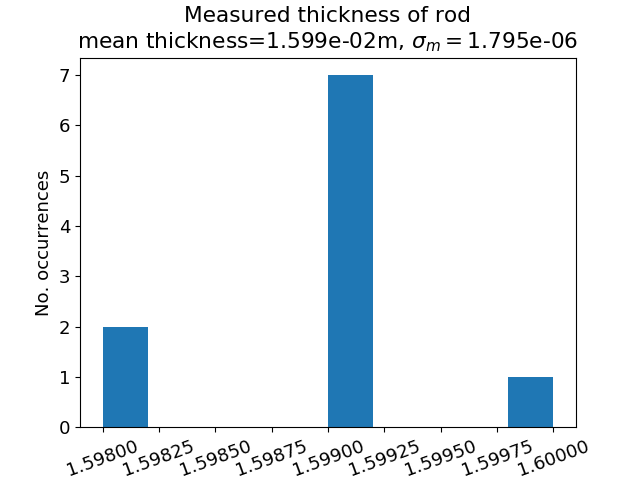
\includegraphics[width=8cm]{scripts/figs/thickdat.png}  
      \caption{Histogram the thickness the of rod measured with micrometer}
      \label{fig:thick} 
    \end{figure} 

    Table \ref{tab:masses} contains all of the masses measured by the balance scale. The stated mass of the reference weights (which is assumed to be their true mass) is fitted against its measured values from the balance scale using a least square fit, the gradient and zero point from this fit is used to calibrate the rough weights and rod, and the corrected masses are given in table \ref{tab:masses_calibrated}.
    \newline
    \newline
    In Fig. \ref{fig:thick} the thickness of the brass rod, measured with a micrometer is shown as a histogram. The mean thickness from this data is $d=15.99\,$mm with a standard deviation $\sigma_m = 1.8\,\mu \textup{m}$
    \newline
    The length of the brass rod measured with the measuring tape, $L=144.4\pm 0.1\,\textup{cm}$ and the length between the two knives in the three-point flex test was measured in two parts, $l_{knife}=4.091\pm 0.001\,\textup{mm}$ and $l_{BC,\,outer}=0.1cm$. (See Fig. \ref{fig:aparatus1})





  \subsection{Results from Three-point flexural test}


    \begin{table}[H]
      % Measured flex
      \caption{Deflection of rod}
      \center
      \begin{tabular}{ | p{1.2cm} | p{1.4cm} | p{1.4cm} | p{1.4cm} | p{1.4cm} | p{1.4cm} | p{1.4cm} | p{1.4cm} | p{1.4cm} |}
          \hline
          Attempt no. & h(0kg) [mm] & h(0.5kg) [mm] & h(1kg) [mm] & h(1.5kg) [mm] & h(2.0kg) [mm] & h(2.5kg) [mm] & h(3.0kg) [mm] & h(3.5kg) [mm] \\ 
          \hline
          1 & 9.44 & 8.72 & 8.00 & 7.28 & 6.58 & 5.84 & 5.15 & 4.43\\ \hline
          2 & 9.42 & 8.70 & 7.98 & 7.26 & 6.53 & 5.80 & 5.09 & 4.39\\ \hline
          3 & 9.42 & 8.71 & 7.98 & 7.26 & 6.53 & 5.80 & 5.09 & 4.37\\ \hline
          4 & 9.41 & 8.69 & 7.97 & 7.25 & 6.52 & 5.79 & 5.08 & 4.36\\ \hline
          5 & 9.42 & 8.70 & 7.98 & 7.26 & 6.70 & 5.87 & 5.19 & 4.51\\ \hline
      \end{tabular}
      \label{tab:flex}
    \end{table}

   
    \begin{figure}[H]
      \centering
      \subfloat[][Deflection of rod]{
        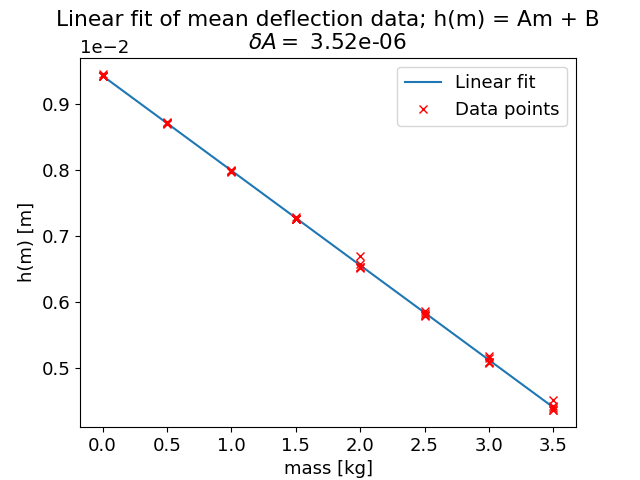
\includegraphics[width=8cm]{scripts/figs/h_m_fig.png}
          \label{fig:h(m)}} 
      \subfloat[][Standard deviation of data]{
        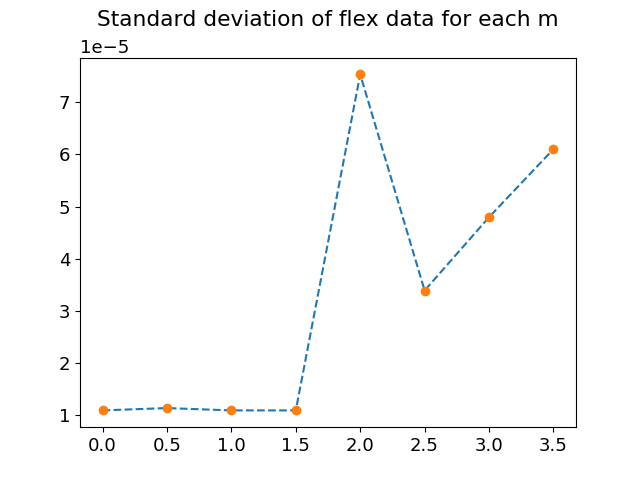
\includegraphics[width=8cm]{scripts/figs/h_m_deviation.png}
          \label{fig:deviation_h_m}}
      \center
      \caption{(a) Shows the deflection of the brass rod measured by the dial gauge. (b) Shows the standard deviation of the data points in (a) at their respective masses}
      \label{fig:exp_1}
    \end{figure}

  Table \ref{tab:flex} contains the deflection data recorded with the dial gauge where the loads listed are from the rough, uncalibrated masses. Their corrected value is listed in table \ref{tab:masses_calibrated}. 
  \newline
  \newline
  Fig. \ref{fig:h(m)} contains all the recorded data, as well as a linear fit on the mean deflection for each load using corrected values for the mass, m. The error of the linear fit, $h(m) = Am + B$, $dA = 3.52e-06$. Fig. \ref{fig:deviation_h_m} contains the standard deviation of the deflection values for each load.
  \newline
  \newline
  From the stated data and their given uncertainties, using Eqn. \ref{eqn:E_deflection} as well as summing the error, the Young's modulus determined by deflection is as follows
  \begin{equation}
    E_{deflection} = 105.8 \pm 0.4\% \, \textup{G}\textup{Pa}
  \end{equation}

  \subsection{Results from measuring the speed of sound in the rod}

    When hearing for beats, me and my lab-partner decided that the root frequency was $\approx 1240\enspace\textup{Hz}$ by the method described in the experimental section. This leads to the following, approximate value of youngs modulus;
    \begin{equation}
      E_{beats} = 108\,\textup{GPa}
    \end{equation}
    \newline
    \begin{figure}[H]
      \centering
      \subfloat[][Time domain]{
        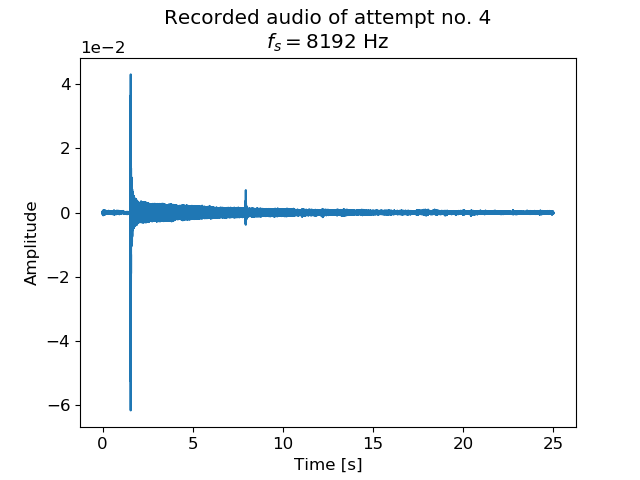
\includegraphics[width=8cm]{scripts/raw_exp2_4.png}
          \label{ }} 
      \subfloat[][Frequency domain]{
        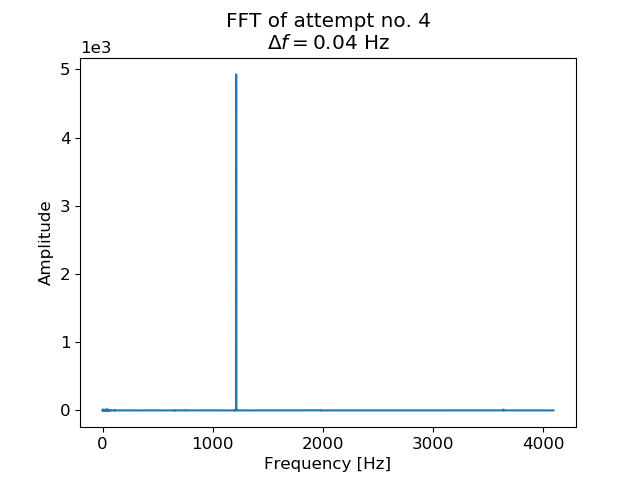
\includegraphics[width=8cm]{scripts/energy_exp2_4.png}
          \label{ }} \\
      \subfloat[][Zoomed frequency domain]{
        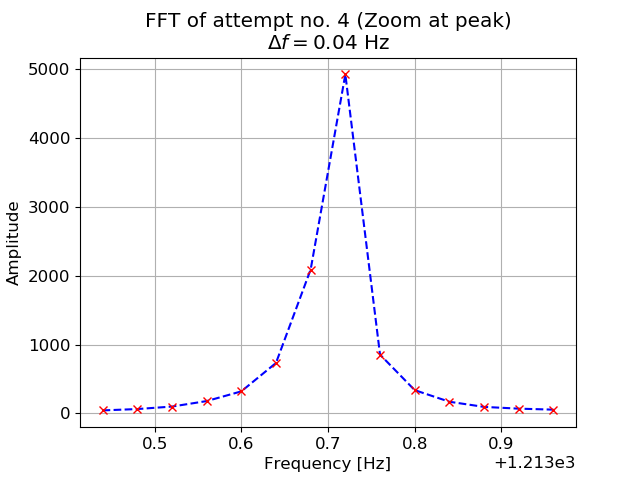
\includegraphics[width=8cm]{scripts/freq_exp2_4.png}
          \label{ }}
      \caption{All of the plots generated for attempt no. 4}
      \label{fig:sound_exp1}
    \end{figure}

    \begin{figure}[H]
      \centering 
      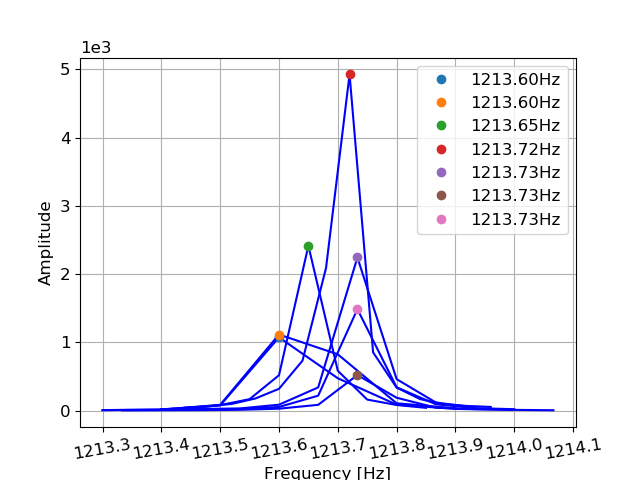
\includegraphics[width=8cm]{scripts/freq_exp2_all.png}
      \caption{Zoomed frequency plot for all 7 attempts.}
      \label{fig:sound_all}
    \end{figure}
    
    Fig. \ref{fig:sound_exp1} contains the data and derived results from our fourth attempt of the experiment. We performed a total of 7 attempts, all of which yielded in similar results to attempt no. 4. The data yielded from all of the attempts is summarized in Fig. \ref{fig:sound_all} which shows the peaks in the frequency domain in one plot.
    Table \ref{tab:fftdat} contains all of the relevant numbers related to each attempt, where $f$ denotes the root frequency, $\Delta f$ the resolution of the frequency domain, $t$ the time of the recording and $f_s$ the sampling frequency.


    \begin{table}[H]
      % FFT DATA
      \center
      \caption{FFT data}
      \begin{tabular}{ | l | p{1.4cm} | l | l | l |}
          \hline
          Attempt no. & $f$ [Hz] & $\Delta f$ [Hz] & $t$ [s] & $f_s$ [Hz]\\ \hline
          1 & 1213.60 & 0.10 & 10 & 8192\\ \hline
          2 & 1213.60 & 0.10 & 10 & 8192\\ \hline
          3 & 1213.65 & 0.05 & 20 & 8192\\ \hline
          4 & 1213.72 & 0.04 & 25 & 8192\\ \hline
          5 & 1213.72 & 0.04 & 25 & 8192\\ \hline
          6 & 1213.72 & 0.07 & 15 & 8192\\ \hline
          7 & 1213.73 & 0.07 & 15 & 8192\\ \hline
      \end{tabular}
      \label{tab:fftdat}
    \end{table}

    Using the root frequency gathered from attempt 4 and 5 (which are identical), the Young's modulus, using Eqn. \ref{eqn:root_tone} is
    \begin{equation}
      E_{sound} = 103.7 \pm 0.2 \% \,\textup{G}\textup{Pa}
    \end{equation}


\newpage
\section{\label{sect:discussion}Discussion}
  For the two independently measured values of Young's modulus to be in agreement with each other, one would expect the difference, $|D|=E_{sound} - E_{deflection}$ to be less than two times the uncertainty of the difference, $s_D$. For the calculated values of $E_{deflection},E_{sound}$, the absolute value of the difference divided by the uncertainty of the difference; $|D|/s_D = 5.3$. Implying that either both, or at least one of the measured values of E is incorrect.
  \newline
  \newline
  Initially, my biggest worry for a systematic error were in the measurements made of the deflection of the beam, however, the uncertainty of $A$, $dA$ was sufficiently small, and not the largest of the accounted for errors in that part of the experiment (which was $l_{BC, outer}$). There may be other systematic errors which I have not thought of, but it seems unlikely.
  \newline
  \newline
  The Young's' modulus measured by beats and recording on the other hand, I have much less information about. The method of listening for beats, if quite obviously flawed and should only serve as an approximation as it is based on the judgment of whomever is listening and therefore quite prone to human error. But as far as the recording is concerned, I know very little about the accuracy of the microphone even though it was quite consistent between attempts. Could perhaps the frequency recorded by the microphone be shifted a bit? The recorded frequency being shifted down compared to the the actual frequency could be a possible explanation as to why there isn't overlap. But this is purely speculation on my part, as I did not make a recording of a known frequency to test the validity of the recorded frequency by.

\section{\label{sect:conclusion}Conclusion}
  In conclusion, I can not with any certainty decide on which of the methods yielded the most accurate result nor if they were both flawed in some fashion. For this, more a closer look at the accuracy of the recorded audio data would be helpful. The results do however point to the value of $E$ for the brass rod being in the range 103.7GPa - 108GPa ($\pm$ uncertainties). But ultimately, more data is required for a more conclusive result, and the results of this report must be taken with a grain of salt due to the potential ramifications of working with an inaccurate value of the Young's modulus.

%%%%%%%%%%%%%%%%%%%%%%%%
%%% END OF MAIN BODY %%%
%%%%%%%%%%%%%%%%%%%%%%%%

\bibliography{rapport3_ref}

\begin{thebibliography}{1}

\bibitem{squires}
G.~L. Squires.
\newblock {\em Practical Physics 4th Edition}.
\newblock Cambridge University Press, 2001.

\bibitem{ymodul}
\url {https://en.wikipedia.org/wiki/Young's_modulus}

\bibitem{beats}
\url{https://en.wikipedia.org/wiki/Beat_(acoustics)#Mathematics_and_physics_of_beat_tones}.

\bibitem{3pt}
\url{https://en.wikipedia.org/wiki/Euler%E2%80%93Bernoulli_beam_theory#Three-point_bending}.

\bibitem{elast}
\url{http://www.uio.no/studier/emner/matnat/fys/FYS2150/v18/kursmateriell/elastisitet/elastisitet.pdf}


\end{thebibliography}

\appendix*
\section{Code}
All of the code used to produce this report are included in this appendix. Included only for the sake of documenting my full work, and was not written with the intention of it being read by anyone. As such it would most likely be rather difficult for anyone (including myself at times) to make sense of it.
\lstinputlisting[language=python]{scripts/FFTlyd.py}
\lstinputlisting[language=python]{scripts/FYS2150lib.py}
\lstinputlisting[language=python]{scripts/lab_data.py}

\end{document}